\section*{4. Проектирование фильтра на диэлектрическом резонаторе (ДР)}

В соответствии с техническим заданием, на выходе созданного малошумящего усилителя необходимо разработать и установить фильтр на основе круглого диэлектрического резонатора. 

В рамках данного этапа была успешно спроектирована геометрическая 3D-модель фильтра в среде электромагнитного моделирования. Конструкция базируется на диэлектрической подложке (относительная диэлектрическая проницаемость 10, толщина 1 мм, размеры 150х150 мм). На поверхности подложки сформированы две микрополосковые линии (МПЛ) передачи шириной 1 мм и длиной 150 мм, выполняющие роль входного и выходного трактов. Между линиями располагается цилиндрический диэлектрический резонатор (также с проницаемостью 10), обеспечивающий частотную селекцию сигнала.

\begin{figure}[H]
	\centering
	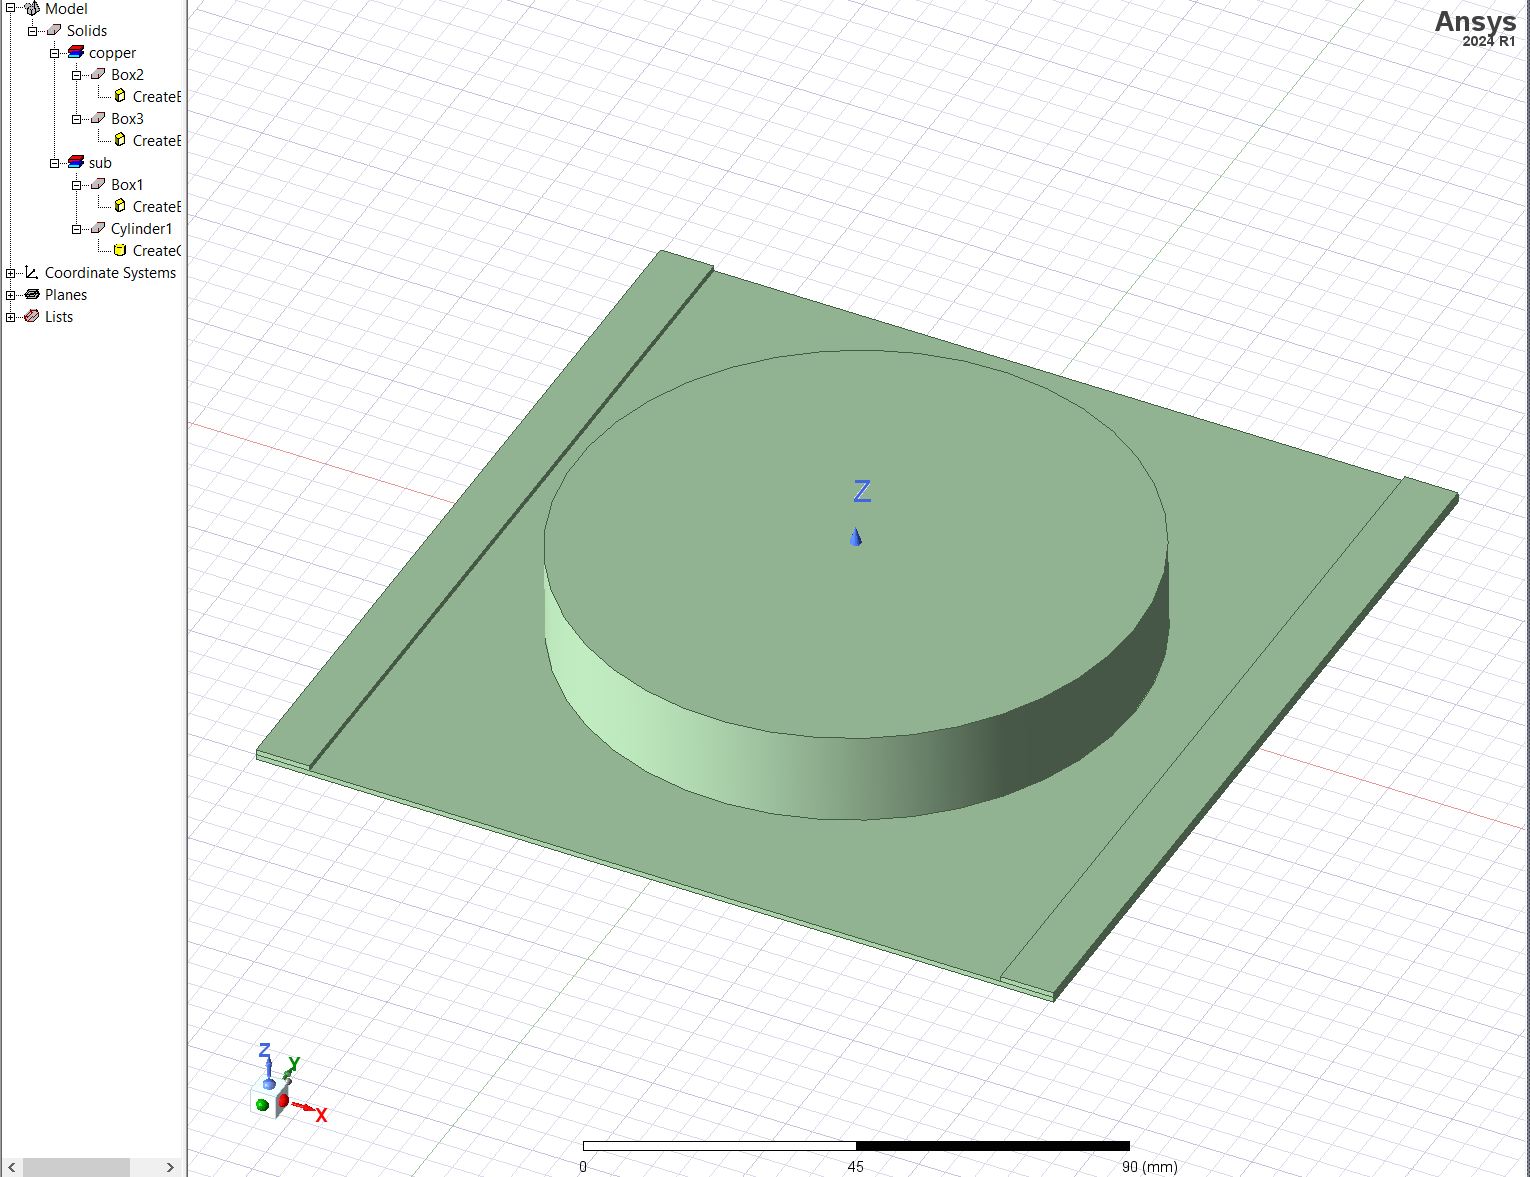
\includegraphics[width=0.8\textwidth]{17.PNG}
	\caption{Трехмерная геометрическая модель фильтра на диэлектрическом резонаторе с микрополосковыми линиями подвода.}
	\label{fig:dr_filter_3d}
\end{figure}

Следует отметить, что в рамках выполнения данного пункта удалось реализовать только пространственное (геометрическое) конструирование подложки, медных линий передачи и самого диэлектрического резонатора. В связи с возникшими техническими сложностями при корректном назначении портов возбуждения на краях микрополосковых линий, произвести полноценный электромагнитный расчет S-параметров спроектированного резонатора не представилось возможным. Как следствие, последующая интеграция модели фильтра в общую схему транзисторного усилителя для проверки увеличения усиления в полосе пропускания (итоговой АЧХ каскада) не была выполнена.